\documentclass[11pt,a4paper]{article}
\usepackage[utf8]{inputenc}
\usepackage[T1]{fontenc}

\usepackage[margin=2cm]{geometry}
\usepackage{xcolor}
\usepackage{enumitem}
\usepackage{booktabs}
\usepackage{tabularx}
\usepackage{fancyhdr}
\usepackage{titlesec}
\usepackage{parskip}
\usepackage{hyperref}
\usepackage{tcolorbox}
\tcbuselibrary{skins,breakable}
\usepackage{tikz}
\usetikzlibrary{positioning,arrows.meta,shapes.geometric,calc,fit,backgrounds}
\usepackage{amsmath}

\definecolor{accent}{HTML}{0f3460}
\definecolor{dark}{HTML}{1a1a2e}
\definecolor{highlight}{HTML}{e94560}
\definecolor{softblue}{HTML}{e8f0fe}
\definecolor{softgreen}{HTML}{e8f5e9}
\definecolor{midgray}{HTML}{666666}
\definecolor{nodeblue}{HTML}{2196F3}
\definecolor{nodegreen}{HTML}{4CAF50}
\definecolor{nodeorange}{HTML}{FF9800}
\definecolor{nodered}{HTML}{e94560}
\definecolor{nodepurple}{HTML}{7E57C2}
\definecolor{clientbg}{HTML}{FFF8E1}

\hypersetup{colorlinks=true,linkcolor=accent,urlcolor=accent}

\titleformat{\section}{\Large\bfseries\color{accent}}{}{0em}{}[\vspace{-0.5em}\textcolor{accent}{\rule{\textwidth}{0.6pt}}]
\titleformat{\subsection}{\large\bfseries\color{dark}}{}{0em}{}

\pagestyle{fancy}
\fancyhf{}
\fancyhead[L]{\small\textcolor{gray}{XC Gradient --- Arquitectura Tècnica}}
\fancyhead[R]{\small\textcolor{gray}{Confidencial}}
\fancyfoot[C]{\small\textcolor{gray}{\thepage}}
\renewcommand{\headrulewidth}{0.4pt}

\newtcolorbox{ipbox}[1][]{
  colback=softblue,colframe=accent,
  fonttitle=\bfseries,
  boxrule=0.4pt,left=6pt,right=6pt,top=4pt,bottom=4pt,#1
}

\begin{document}

\begin{center}
{\Huge\bfseries\color{dark} Arquitectura Tècnica}\\[0.3em]
{\Large\color{accent} XC Gradient --- Visió General del Sistema}\\[0.5em]
{\small\color{midgray} Abril 2026 $\cdot$ Confidencial}
\end{center}

\vspace{0.5em}
{\color{accent}\hrule height 1pt}
\vspace{1em}

\section{1. Visió d'Alt Nivell}

El sistema XC Gradient transforma documentació industrial no estructurada en respostes accionables mitjançant un pipeline d'IA completament privat. Cap dada del client abandona les seves instal·lacions.

\vspace{0.5em}

\begin{center}
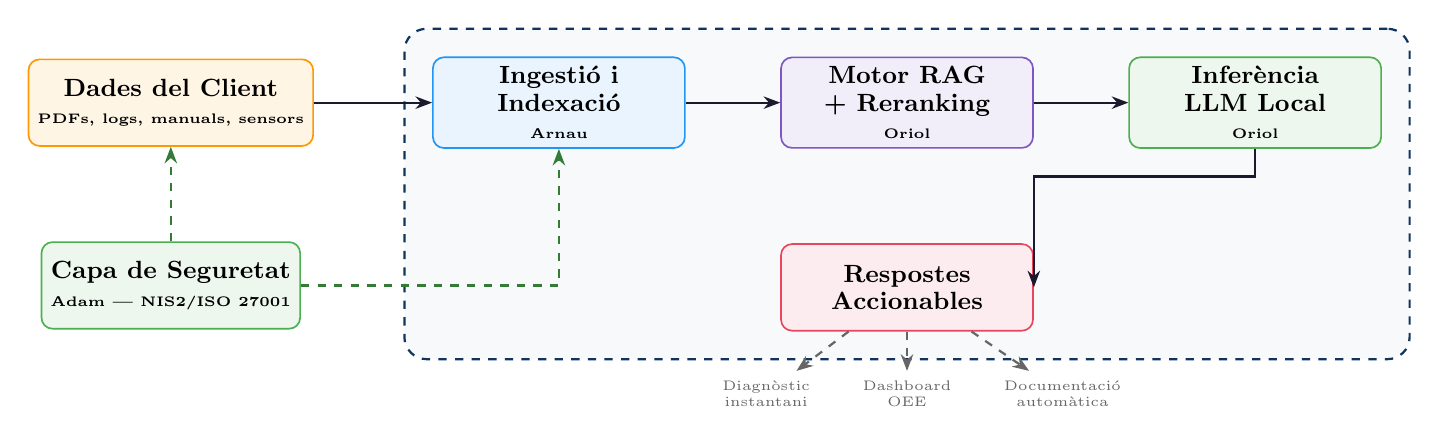
\begin{tikzpicture}[
  node distance=0.6cm and 1.2cm,
  block/.style={rectangle, rounded corners=4pt, draw=#1, fill=#1!10, 
    minimum width=3.2cm, minimum height=1.1cm, align=center,
    font=\small\bfseries, line width=0.6pt},
  arrow/.style={-{Stealth[length=6pt]}, thick, color=dark},
  label/.style={font=\tiny\color{midgray}, align=center}
]

% Row 1: Input
\node[block=nodeorange] (input) {Dades del Client\\[-0.1em]\tiny PDFs, logs, manuals, sensors};

% Row 2: Processing
\node[block=nodeblue, right=1.5cm of input] (ingest) {Ingestió i\\[-0.1em]Indexació\\[-0.1em]\tiny Arnau};
\node[block=nodepurple, right=1.2cm of ingest] (rag) {Motor RAG\\[-0.1em]+ Reranking\\[-0.1em]\tiny Oriol};
\node[block=nodegreen, right=1.2cm of rag] (llm) {Inferència\\[-0.1em]LLM Local\\[-0.1em]\tiny Oriol};

% Row 3: Output  
\node[block=nodered, below=1.2cm of rag] (output) {Respostes\\[-0.1em]Accionables};

% Outputs detail
\node[label, below left=0.5cm and -0.5cm of output] (o1) {Diagnòstic\\instantani};
\node[label, below=0.5cm of output] (o2) {Dashboard\\OEE};
\node[label, below right=0.5cm and -0.5cm of output] (o3) {Documentació\\automàtica};

% Security wrapper
\node[block=nodegreen, below=1.2cm of input, minimum width=2.8cm] (sec) {Capa de Seguretat\\[-0.1em]\tiny Adam --- NIS2/ISO 27001};

% Arrows
\draw[arrow] (input) -- (ingest);
\draw[arrow] (ingest) -- (rag);
\draw[arrow] (rag) -- (llm);
\draw[arrow] (llm.south) -- ++(0,-0.35) -| (output.east);
\draw[arrow,dashed,color=midgray] (output) -- (o1);
\draw[arrow,dashed,color=midgray] (output) -- (o2);
\draw[arrow,dashed,color=midgray] (output) -- (o3);

% Security connections
\draw[arrow, dashed, color=nodegreen!70!black] (sec.north) -- (input.south);
\draw[arrow, dashed, color=nodegreen!70!black] (sec.east) -| (ingest.south);

% Container label
\begin{scope}[on background layer]
\node[draw=accent, dashed, thick, rounded corners=8pt, 
  fit=(ingest)(rag)(llm)(output), 
  inner sep=10pt, fill=accent!3,
  label={[font=\footnotesize\color{accent}\bfseries]above:Contenidor Privat del Client (aïllat)}] {};
\end{scope}

\end{tikzpicture}
\end{center}

\vspace{0.3em}

\begin{ipbox}
\textbf{Principi fonamental:} cada client disposa d'un contenidor privat aïllat. La inferència del model de llenguatge s'executa localment dins les instal·lacions del client. Zero dependència de proveïdors d'IA externs (OpenAI, Azure, Google).
\end{ipbox}

\section{2. Arquitectura Detallada per Capa}

\subsection{2.1~~Capa d'Ingestió i Indexació \textnormal{\small (Propietari: Arnau Noguer, CTO)}}

Processa tota la documentació del client i la converteix en un índex consultable:

\begin{itemize}[leftmargin=1.5em,itemsep=2pt]
\item \textbf{Pipeline d'ingestió:} PDFs, fitxers Word, logs de manteniment, dades de sensors i registres d'incidents es processen, segmenten i indexen.
\item \textbf{Recuperació híbrida:} combinació de cerca densa (embeddings vectorials) i dispersa (BM25) sobre el vector store privat del client.
\item \textbf{Construcció d'ontologia:} mapa conceptual del domini manufacturerer del client --- tipus de màquina, modes de fallada, famílies de paràmetres. Aquesta ontologia es refina amb cada desplegament i crea costos de canvi creixents.
\item \textbf{Vector store aïllat:} un índex per client, mai compartit entre comptes.
\end{itemize}

\subsection{2.2~~Capa de Post-Recuperació \textnormal{\small (Propietari: Oriol Farrés, CEO --- IP de Tesi)}}

Optimitza la selecció del context que rep el model de llenguatge. Aquí resideix la IP core:

\begin{ipbox}[title={\color{accent}IP Propietària: Formalització Markov + Choquet}]
El pas de recuperació retorna $n$ chunks candidats. El reranker selecciona la finestra de context òptima.

\textbf{Cadena de Markov absorbent:} el pipeline RAG es formalitza com una cadena de Markov sobre conjunts de documents candidats, on cada transició representa una operació de reranking.

\textbf{Integral de Choquet:} les transicions de reranking s'avaluen mitjançant un framework de teoria de jocs (integral de Choquet sobre un DAG proposicional) que captura \textit{sinergies i redundàncies} entre chunks --- una capacitat que els mètodes de scoring additius no poden oferir.

\textbf{Restricció de latència:} $<$50ms en CPU per reranking, compatible amb desplegament on-premises sense cluster GPU.
\end{ipbox}

\subsection{2.3~~Capa d'Inferència del Model \textnormal{\small (Propietari: Oriol Farrés, CEO --- IP de Tesi)}}

El model de llenguatge genera la resposta final a partir del context optimitzat:

\begin{itemize}[leftmargin=1.5em,itemsep=2pt]
\item \textbf{S-QDoRA (Sparse Quantized DoRA):} mètode de fine-tuning multi-tenant que dóna a cada client un adaptador dispers lleuger sobre un model base quantitzat compartit. Permet especialització per client sense emmagatzemar un model complet per client.
\item \textbf{Speculative decoding:} un model petit ``draft'' genera tokens candidats que el model objectiu verifica en paral·lel, aconseguint reducció de latència de 2--4$\times$ --- crític per a desplegaments sense accés a clusters GPU.
\item \textbf{Inferència local:} dual RTX 3090 (48GB VRAM total) permet executar models quantitzats de 70B paràmetres.
\end{itemize}

\subsection{2.4~~Capa de Seguretat i Topologia \textnormal{\small (Propietari: Adam Sarrate, COO/CISO)}}

\begin{itemize}[leftmargin=1.5em,itemsep=2pt]
\item \textbf{Topologia de xarxa:} defineix com la capa XC Gradient s'integra dins la infraestructura existent del client --- què es connecta a què, on viu el contenidor privat, com els operaris accedeixen al node d'inferència.
\item \textbf{Aïllament entre clients:} garanties d'aïllament estricte, control d'accés al contenidor privat, i model de flux de dades que assegura que cap dada arriba a proveïdors externs.
\item \textbf{Conformitat:} arquitectura dissenyada per complir NIS2 (UE 2022/2555) i ISO~27001 de sèrie.
\end{itemize}

\section{3. Framework d'Avaluació}

Per garantir la qualitat de les respostes, XC Gradient utilitza un framework de benchmarking propi que supera les limitacions de RAGAS:

\begin{center}
\renewcommand{\arraystretch}{1.2}
\small
\begin{tabularx}{0.92\textwidth}{l X}
\toprule
\textbf{Component} & \textbf{Descripció} \\
\midrule
BERTScore (DeBERTa) & Similitud semàntica entre resposta generada i referència \\
NLI asimètric & Verificació d'entailment i contradicció \\
Cross-encoder & Rellevància entre consulta i resposta \\
Jutge LLM (70B) & Avaluació estructurada en una sola crida \\
\midrule
\textbf{Mètode} & Ensemble lineal de 7 features, ajustat contra 200 exemples anotats per humans \\
\textbf{Objectiu} & A-score $>$0.80 al PoC de Decfa (Arnau, target: 15 maig 2026) \\
\textbf{Protocol estadístic} & Wilcoxon signed-rank amb correcció de Bonferroni, pre-registrat \\
\bottomrule
\end{tabularx}
\end{center}

\section{4. Diferenciació Tècnica vs. Estat de l'Art}

\begin{center}
\renewcommand{\arraystretch}{1.3}
\begin{tabularx}{0.92\textwidth}{X c c}
\toprule
\textbf{Capacitat} & \textbf{RAG Estàndard} & \textbf{XC Gradient} \\
\midrule
Reranking & Scoring additiu (lineal) & Choquet integral (captura sinergies) \\
Multi-tenancy & Un model per client (costós) & S-QDoRA: adaptadors dispersos compartint base \\
Latència & Estàndard & Speculative decoding (2--4$\times$ reducció) \\
Privacitat & Cloud-dependent & 100\% on-premises, zero exfiltració \\
Domini & Genèric & Ontologies industrials per client \\
Avaluació & RAGAS (limitat) & Ensemble 7-features calibrat amb humans \\
\bottomrule
\end{tabularx}
\end{center}

\section{5. Stack Tecnològic}

\begin{center}
\renewcommand{\arraystretch}{1.2}
\small
\begin{tabularx}{0.92\textwidth}{l X}
\toprule
\textbf{Capa} & \textbf{Tecnologies} \\
\midrule
Inferència & Models quantitzats 70B, dual RTX 3090, speculative decoding \\
Retrieval & Vector store aïllat per client, cerca híbrida densa+dispersa \\
Reranking & Pipeline Markov+Choquet (C++/Python, $<$50ms CPU) \\
Fine-tuning & S-QDoRA amb hot-swap d'adaptadors LoRA \\
Backend & Python, FastAPI \\
Frontend & React, dashboard OEE 2D interactiu \\
Seguretat & Contenidors aïllats, NIS2/ISO~27001 compliant \\
DevOps & Kubuntu 24.04, Tailscale per accés remot \\
\bottomrule
\end{tabularx}
\end{center}

\vfill
\begin{center}
\small\textcolor{midgray}{XC Gradient $\cdot$ Arquitectura Tècnica $\cdot$ Confidencial $\cdot$ Abril 2026}
\end{center}

\end{document}
